\section{Transaction Contracts}

While contracts on individual operations offer the programmer object-level
declarative reasoning, real-world scenarios often involve operations that span
multiple objects. In order to address this problem, several recent
systems~\cite{COPS,BurckhardtESOP,BailisHAT} have proposed a variety of
transactions, with varying semantics, in order to compose operations on
multiple objects. However, given that classical transaction models such as
serializability~\cite{} and snapshot isolation~\cite{} require inter-replica
coordination, these systems espouse \emph{coordination-free transactions} that
remain available under network partitions, but only provide weaker isolation
guarantees. Coordination-free transactions have intricate consistency semantics
and widely varying runtime overheads. As with operation-level consistency, the
onus is on the programmer to pick the correct transaction kind, the choice of
which is complicated by the consistency requirement of the operations it
composes.

\subsection{Syntax and Semantics Extension}
\label{sec:syn_sem_ext}

\name automates the choice of assigning the correct and most efficient
transaction isolation level. Similar to contracts on individual operations, the
programmer associates contracts with transactions, declaratively expressing its
consistency specification. We extend the contract language with a new term
under quantifier-free propositions ${\small \txnZ}~S_1~S_2$, where $S_1$ and
$S_2$ are sets of effects, and introduce a new primitive equivalence relation
$\small \sametxnZ$ that holds for effects from the same transaction. $\small
\txn{a,b}{c,d}$ is just syntactic sugar for $\small \sametxn{a}{b} ~\wedge~
\sametxn{c}{d} ~\wedge~ \neg\sametxn{a}{c}$, where $a$ and $b$ considered to
belong to the \emph{current} transaction.

We assume that operations not part of any transaction to belong to their own
unique transaction. While the transactions may have varying isolation
guarantees, we make the standard assumption that all transactions provide
atomicity. Hence, we include the following axiom in $\Delta$: $\small \forall
a,b,c.~\txn{a}{b,c} ~\wedge~ \sameobj{b}{c} ~\wedge~ \vis{b}{a} \Rightarrow
\vis{c}{a}$. The semantics of this contract is illustrated represented in
Figure~\ref{fig:txn_atomicity}.

\subsection{Transactional Bank Account}

In order to illustrate the utility of declarative reasoning for transactions,
let us extend our running bank account example with use two accounts (objects)
-- current ($c$) and savings ($s$). Each account provides operations
\cf{withdraw}, \cf{deposit} and \cf{getBalance}, with the same contracts as
defined previously. We consider two transactions -- \cf{save(amt)}, which
transfers \cf{amt} from current to savings, and \cf{totalBalance} returns the
sum of the balances of individual accounts. The \name code for the transactions
is given below:
\vspace{-1em}

\noindent \begin{minipage}[t]{0.5\columnwidth}
\begin{codehaskell}
save amt =
  x <- $(classify psi1)
  atomically x $ do
    b <- withdraw c amt
    when b $ deposit s amt
\end{codehaskell}
\end{minipage}
\begin{minipage}[t]{0.5\columnwidth}
\begin{codehaskell}
totalBalance =
  x <- $(classify psi2)
  atomically x $ do
    b1 <- getBalance s
    b2 <- getBalance s
    return b1 + b2
\end{codehaskell}
\end{minipage}

\noindent $\cv_1$ and $\cv_2$ are the contracts on the corresponding
transactions. Our goal is to ensure that \cf{totalBalance} returns the result
obtained from a consistent snapshot of the object states.

While making both transactions serializable would ensure correctness,
distributed stores rarely offer serializable transactions. Moreover,
serializability is unavailable and hinders scalability. As we will see, these
transactions can be satisfied with much weaker isolation guarantees. Despite
the atomicity offered by the transaction, anomalies are still possible. For
example, the two \cf{getBalance} operations in \cf{totalBalance} transactions
might be served by different replicas with distinct set of committed \cf{save}
transactions. If the first(second) \cf{getBalance} operation witness a
\cf{save} transaction that is not witnessed by the second(first)
\cf{getBalance} operation, then the balance returned will be less(greater) than
the actual balance. It is not immediately apparent which weakest isolation
guarantee will be sufficient to prevent the anomaly.

Instead, \name requires the programmer to simply state the consistency
requirement as a contract. Since we would like both the \cf{getBalance}
operations to witness the same set of \cf{save} transactions, we define the
constraint on \cf{totalBalance} transaction $\psi_2$ as:

\vspace{-1em}
\begin{smathpar}
\begin{array}{l}
\cv_{2} = \forall a:\rcf{getBalance}, b:\rcf{getBalance}, \\
\qquad (c:\rcf{withdraw} \vee \rcf{deposit}), (c:\rcf{withdraw} \vee \rcf{deposit}). \\
\qquad \txn{a,b}{c,d} ~\wedge~ \vis{c}{a} ~\wedge~ \sameobj{d}{b} \Rightarrow \vis{d}{b}
\end{array}
\end{smathpar}

\noindent The key idea in the above definition is that the $\txnZ$ primitive
allows us to relate operations on different objects.

The \cf{save} transaction only needs to ensure that the two writes it performs
are made visible atomically. Since this is ensured by combining them in a
transaction, \cf{save} does not require any additional constraints, and
$\psi_1$ is simply $\small \true$.

\subsection{Coordination-free Transactions}

\begin{figure}
\centering
\subfigure[Atomicity]{\label{fig:txn_atomicity}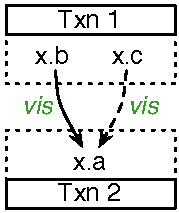
\includegraphics[width=0.25\columnwidth]{Figures/TxnAtomic}}
\hfill
\subfigure[Monotonic Atomic View]{\label{fig:txn_mav}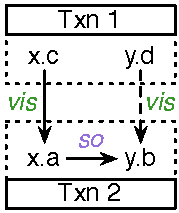
\includegraphics[width=0.25\columnwidth]{Figures/TxnMAV}}
\hfill
\subfigure[Repeatable Read]{\label{fig:txn_rr}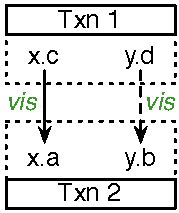
\includegraphics[width=0.25\columnwidth]{Figures/TxnRR}}
\caption{Semantics of transaction contracts. $x$ and $y$ are distinct objects.
The dotted line represents the visibility requested by the contracts.}
\label{fig:transaction}
\end{figure}

In order to illustrate the utility of transaction contract classification, we
identify three well-understood coordination-free transaction semantics -- Read
Committed (RC)~\cite{}, Monotonic Atomic View (MAV)~\cite{} and Repeatable Read
(RR)~\cite{}, and illustrate the classification strategy. Our technique can
indeed be applied to a different isolation level lattice.

A transaction with ANSI RC semantics only witnesses committed operations. Let
us assume that the store buffers updates until all the updates from the
transaction are available at a replica. If the transaction commits, the
buffered updates are made visible. Otherwise, the buffered updates are
discarded. In particular, a store implementing RC does not require
inter-replica coordination. RC does not entail any further isolation
guarantees. We can express RC as follows:

\vspace{-1em}
\begin{smathpar}
\rcc = \forall a,b,c.~\txn{a}{b,c} \wedge \sameobj{b}{c} \wedge \vis{b}{a} \Rightarrow \vis{c}{a}
\end{smathpar}

\noindent Notice that the above definition is the same as the atomicity
guarantee of transaction described in Section~\ref{sec:syn_sem_ext}. The
\cf{save} is an example for RC transaction.

MAV semantics ensures that if some operation in a transaction $T_1$ witnesses
the effects of another transaction $T_2$, then subsequent operations in $T_1$
will also witness the effects of $T_2$. MAV semantics is useful for
maintaining the integrity of foreign key constraints, materialized views and
secondary updates. In order to implement MAV, a store only needs to keep track
of the set of transactions $S_t$ witnessed by the running transaction, and
before performing an operation at some replica, ensure that the replica
includes all the transactions in $S_t$. Hence, MAV is coordination-free. MAV
semantics is captured with the following contract:

\vspace{-1em}
\begin{smathpar}
\begin{array}{l}
\mavc = \forall a,b,c,d.~\txn{a,b}{c,d} ~\wedge~ \so{a}{b} ~\wedge~ \vis{c}{a} \\
\qquad\qquad\qquad\qquad ~\wedge~ \sameobj{d}{b} \Rightarrow \vis{d}{b}
\end{array}
\end{smathpar}

\noindent whose semantics is illustrated in the Figure~\ref{fig:txn_mav}.

RR semantics requires that the transaction witness a snapshot of the data store
state. Importantly, this snapshot can be obtained from any replica, and hence
RR is coordination-free. An example for such a transaction is the
\cf{totalBalance} transaction. The semantics of RR is captured by the following
contract:

\vspace{-1em}
\begin{smathpar}
\begin{array}{l}
\rrc = \forall a,b,c,d.~\txn{a,b}{c,d} ~\wedge~ \vis{c}{a} \\
\qquad\qquad\qquad\quad ~\wedge~ \sameobj{d}{b} \Rightarrow \vis{d}{b}
\end{array}
\end{smathpar}

\noindent whose semantics is illustrated in the Figure~\ref{fig:txn_rr}.

\subsection{Classification}

Similar to operation-level contracts, with respect to $\le$ relation, the
coordination-free transaction semantics described here form a total order:
$\rcc \le \mavc \le \rrc$. The transaction classification is also similar to
the operation-level contract classification presented in
Figure~\ref{sem:classify}; given a contract $\psi$ on a transaction, we start
from the weakest transaction contract $\rcc$, and progressively compare its
strength to the known transaction contracts until we find a isolation level
under which $\psi$ can be safely discharged. Otherwise, we report a type error.
